% !Mode:: "TeX:UTF-8"
% !BIB program = bibtex
% !TEX program = xelatex

% \documentclass[withoutpreface,bwprint,ebook]{../../../Template/cumcmthesis} % 普通草稿
% \documentclass[draft,ebook]{../../../Template/cumcmthesis} % 电子书草稿
\documentclass{../../../Template/cumcmthesis-2025} % 带封面的版本
% \documentclass[withoutpreface,bwprint]{../../../Template/cumcmthesis} %去掉封面与编号页

% 基本信息
\title{烟幕干扰弹无人机投放策略优化的数学建模研究} % 文章标题写到这里
\tihao{A}
\baominghao{202508013001}
\schoolname{哈尔滨商业大学}
\membera{邹文杰} % 成员
\memberb{李慧}
\memberc{盛炫皓}
\supervisor{郭丽华}
\yearinput{2025}
\monthinput{9}
\dayinput{7}

% 载入路径
\makeatletter
\def\input@path{{sections/}{figures/}{../../figures/}}
\makeatother

% 导入符号
% % 符号定义文件,命令所有文件共享
% 并在 notations 打印

\glsxtrnewsymbol[
	description={%
		an example symbol % 对符号的描述
	},
	unit={\si{m^2}} % 单位,不显示可以不写
]{e}{\ensuremath{\mathcal{E}}}
% 第一个参数e是后期可以直接\gls{e}代表之后的符号


% 额外引用的宏包
\usepackage{../../../Styles/mystyle-cumcmthesis}
\usepackage{subfiles}  % Best loaded last in the preamble

\begin{document}

% TODO 提交最终版论文时别忘了选择 7,8行版本
% \listoftodos
\maketitle

\subfile{sections/abstract}

\section{问题重述}

\subfile{sections/question_review}



\section{问题的分析}

\subfile{sections/analyse}



\section{模型的假设}

\subfile{sections/assumptions}



\section{符号说明}

\subfile{sections/notations}
\section{模型的建立与求解}

\subsection{问题一}

\subsubsection{问题一的模型建立}

\subfile{sections/q1_build}

\subsubsection{模型求解}

\subfile{sections/q1_solution}

\subsection{问题二}

\subsubsection{模型建立}

\subfile{sections/q2_build}

\subsubsection{模型求解}

\subfile{sections/q2_solution}

\subsection{问题三}

\subsubsection{模型建立}

\subfile{sections/q3_build}

\subsubsection{模型求解}
\subfile{sections/q3_solution}

\subsection{问题四}

\subsubsection{模型建立}

\subfile{sections/q4_build}

\subsubsection{模型求解}
\subfile{sections/q4_solution}

\subsubsection{灵敏度分析}
\subfile{sections/q4_analyse}

\subsection{问题五}

\subsubsection{模型建立}

\subfile{sections/q5_build}

\subsubsection{模型求解}
\subfile{sections/q5_solution}

\section{模型的评价}

\subfile{sections/model_review}

\section{参考文献}

\begingroup
\renewcommand{\section}[2]{}%
% \renewcommand{\chapter}[2]{}% for other classe
\begin{thebibliography}{99}  
\bibitem{ref1}
司守奎,孙玺菁,数学建模算法与应用[M].北京:国防工业出版社,2022 
\bibitem{doubao}
Doubao,1.5-pro,字节跳动,2025-09-05 
\end{thebibliography}
\endgroup
% 参考文献部分

\newpage
\nocite{*}
\bibliography{../reference/reference}


\newpage
\begin{appendices} % 附录

\section{}

\begin{figure}[H]
\centering
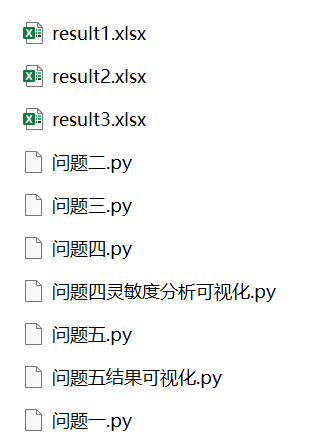
\includegraphics[scale=0.8]{支撑材料文件列表.png}
\end{figure}

\lstinputlisting[language=python]{../src/问题一.py}

\lstinputlisting[language=python]{../src/问题二.py}

\lstinputlisting[language=python]{../src/问题三.py}

\lstinputlisting[language=python]{../src/问题四.py}

\lstinputlisting[language=python]{../src/问题四灵敏度分析可视化.py}

\lstinputlisting[language=python]{../src/问题五.py}

\lstinputlisting[language=python]{../src/问题五结果可视化.py}


% \section{导入其他代码的测试}


\end{appendices}

\end{document}
